\subsection{Software Development}
\subsubsection{Variations from initial plans}
During the sprint that will be discussed in further detail below, it was determined that Python and the Kivy framework were not a fully suitable technology stack for the needs of our application. The python library for visualization that we investigated and used at the beginning of the sprint did not function well with real time updating of data, as well as requiring the environment to be properly set up on each local machine the application would be running on. There was also limited documentation and library options with that technology stack. Due to these limitations, as well as experience as most of the software team having experience with building javascript web application, the decision was made, two days into the spritn to  to shift to building a web application using React framework for JavaScript where, through accessing a webpage on any device connected to the internet, it would be possible to access the GUI. Because of React's prevalence in the web development world, there is an abundance of documentation and libraries to help the the team develop the application that was initially envisioned. 

The role of the web application has also been expanded from original plans. Originally, the application was to serve as a method of monitoring real-time readings only, and all historical data was to be accessed through ThingSpeak. However, the team decided to congregate all data and functionality into one place - being the web application. This further allow the data to be organized the way the team decides is most useful for later data analysis, rather than it being dictated by ThingSpeak's structure. With the addition of the data history page, all data collected will be stored in the application's own database separate from ThingSpeak, and all data will be accessible from the data history page. With this expansion, a host of dropdowns and toggle switches that are set by the end user during operation and keep track of the type of drill, type of activity (skating or shooting), participant, and drill surface (ice or dyland) in order to organize as it passes from ThingSpeak to the application database through our application. 

\subsubsection{Progress}
In the new year, the software team organized a sprint spanning the last nine days of the winter break. The sprint saw the beginning and large progress in the development of the Data Collection and Monitoring Web Application and its data component. 

The team's progress with connecting the data collecting side (Thingspeak) to the front end side has been a large success. Being able to have multiple channels with each have multiple fields has been very helpful for the team. Each type of sensor has been assigned it's own channel, with each sensor within the three types being assigned its own field. For example, the EMG sensors have their own channel, with each of the 6 EMG sensors representing one field in that channel. 
\begin{figure}[htbp]
\centering
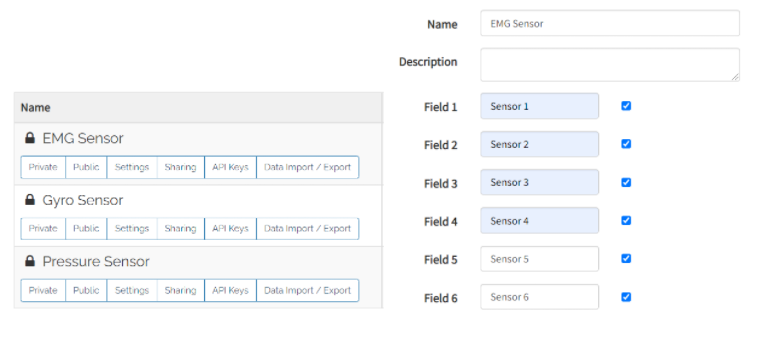
\includegraphics[scale=0.9]{Progress_Report/figs/Thingspeak.png}
\caption{Demonstration of the breakdown of Thingspeak}
\label{fig:ThingSpeak}
\end{figure}

Since the Arduinos that control the sensors will be sending data every one second to their respective channels and fields, the application will be fetching this data every one second as well. Doing so will allow for perfect data collection and visualization. In addition, the team was able to use JavaScript's synchronous nature to their advantage. In doing so, the team was able to avoid the problem of multithreading a web application which could become very messy. The part of the code that fetches the data from Thingspeak will be executed one channel at a time. This is executed so quickly that it mimics the behaviour of multithreading on the front end side and will display every single data point from every single sensor at the same time every one second. 

\paragraph{Data Collection and Monitoring Web App}


The web application's graphical user interface was wire framed, and subsequently built out. The design of the web application would consist of 5 total pages: An overview page where current real-time readings of each sensor can be seen all at once, 1 page for each of the 3 sensor types, that will show a readings table and graph visualizing the readings as they come in. There is also a data history page that will allow the end user to browse all data collected. See [insert section here] of the appendix for the UI wireframe. 

The data collection web application is built using a stack consisting of ReactJS and NodeJS Frameworks. The application was built with a component-based approach, where the construction began by building the components that would be found on the pages of the application. To date, the gauge component that will be displayed on the overview dashboard to display the reading on the host of sensors concurrently collecting data was built. The data table components that will dynamically display incoming readings from individual sensors on their respective pages was built. Also built was the graph component that will graphically and dynamically display individual sensor readings on their respective pages. The team has built out the common frame of the web application consisting of the navigation bar, and filtering options consisting of drop-down, and toggle switches which will allow the end user to input the parameters of the data currently being observed. 

\begin{figure}[h]
     \centering
     \begin{subfigure}[h]{0.45\textwidth}
         \centering
         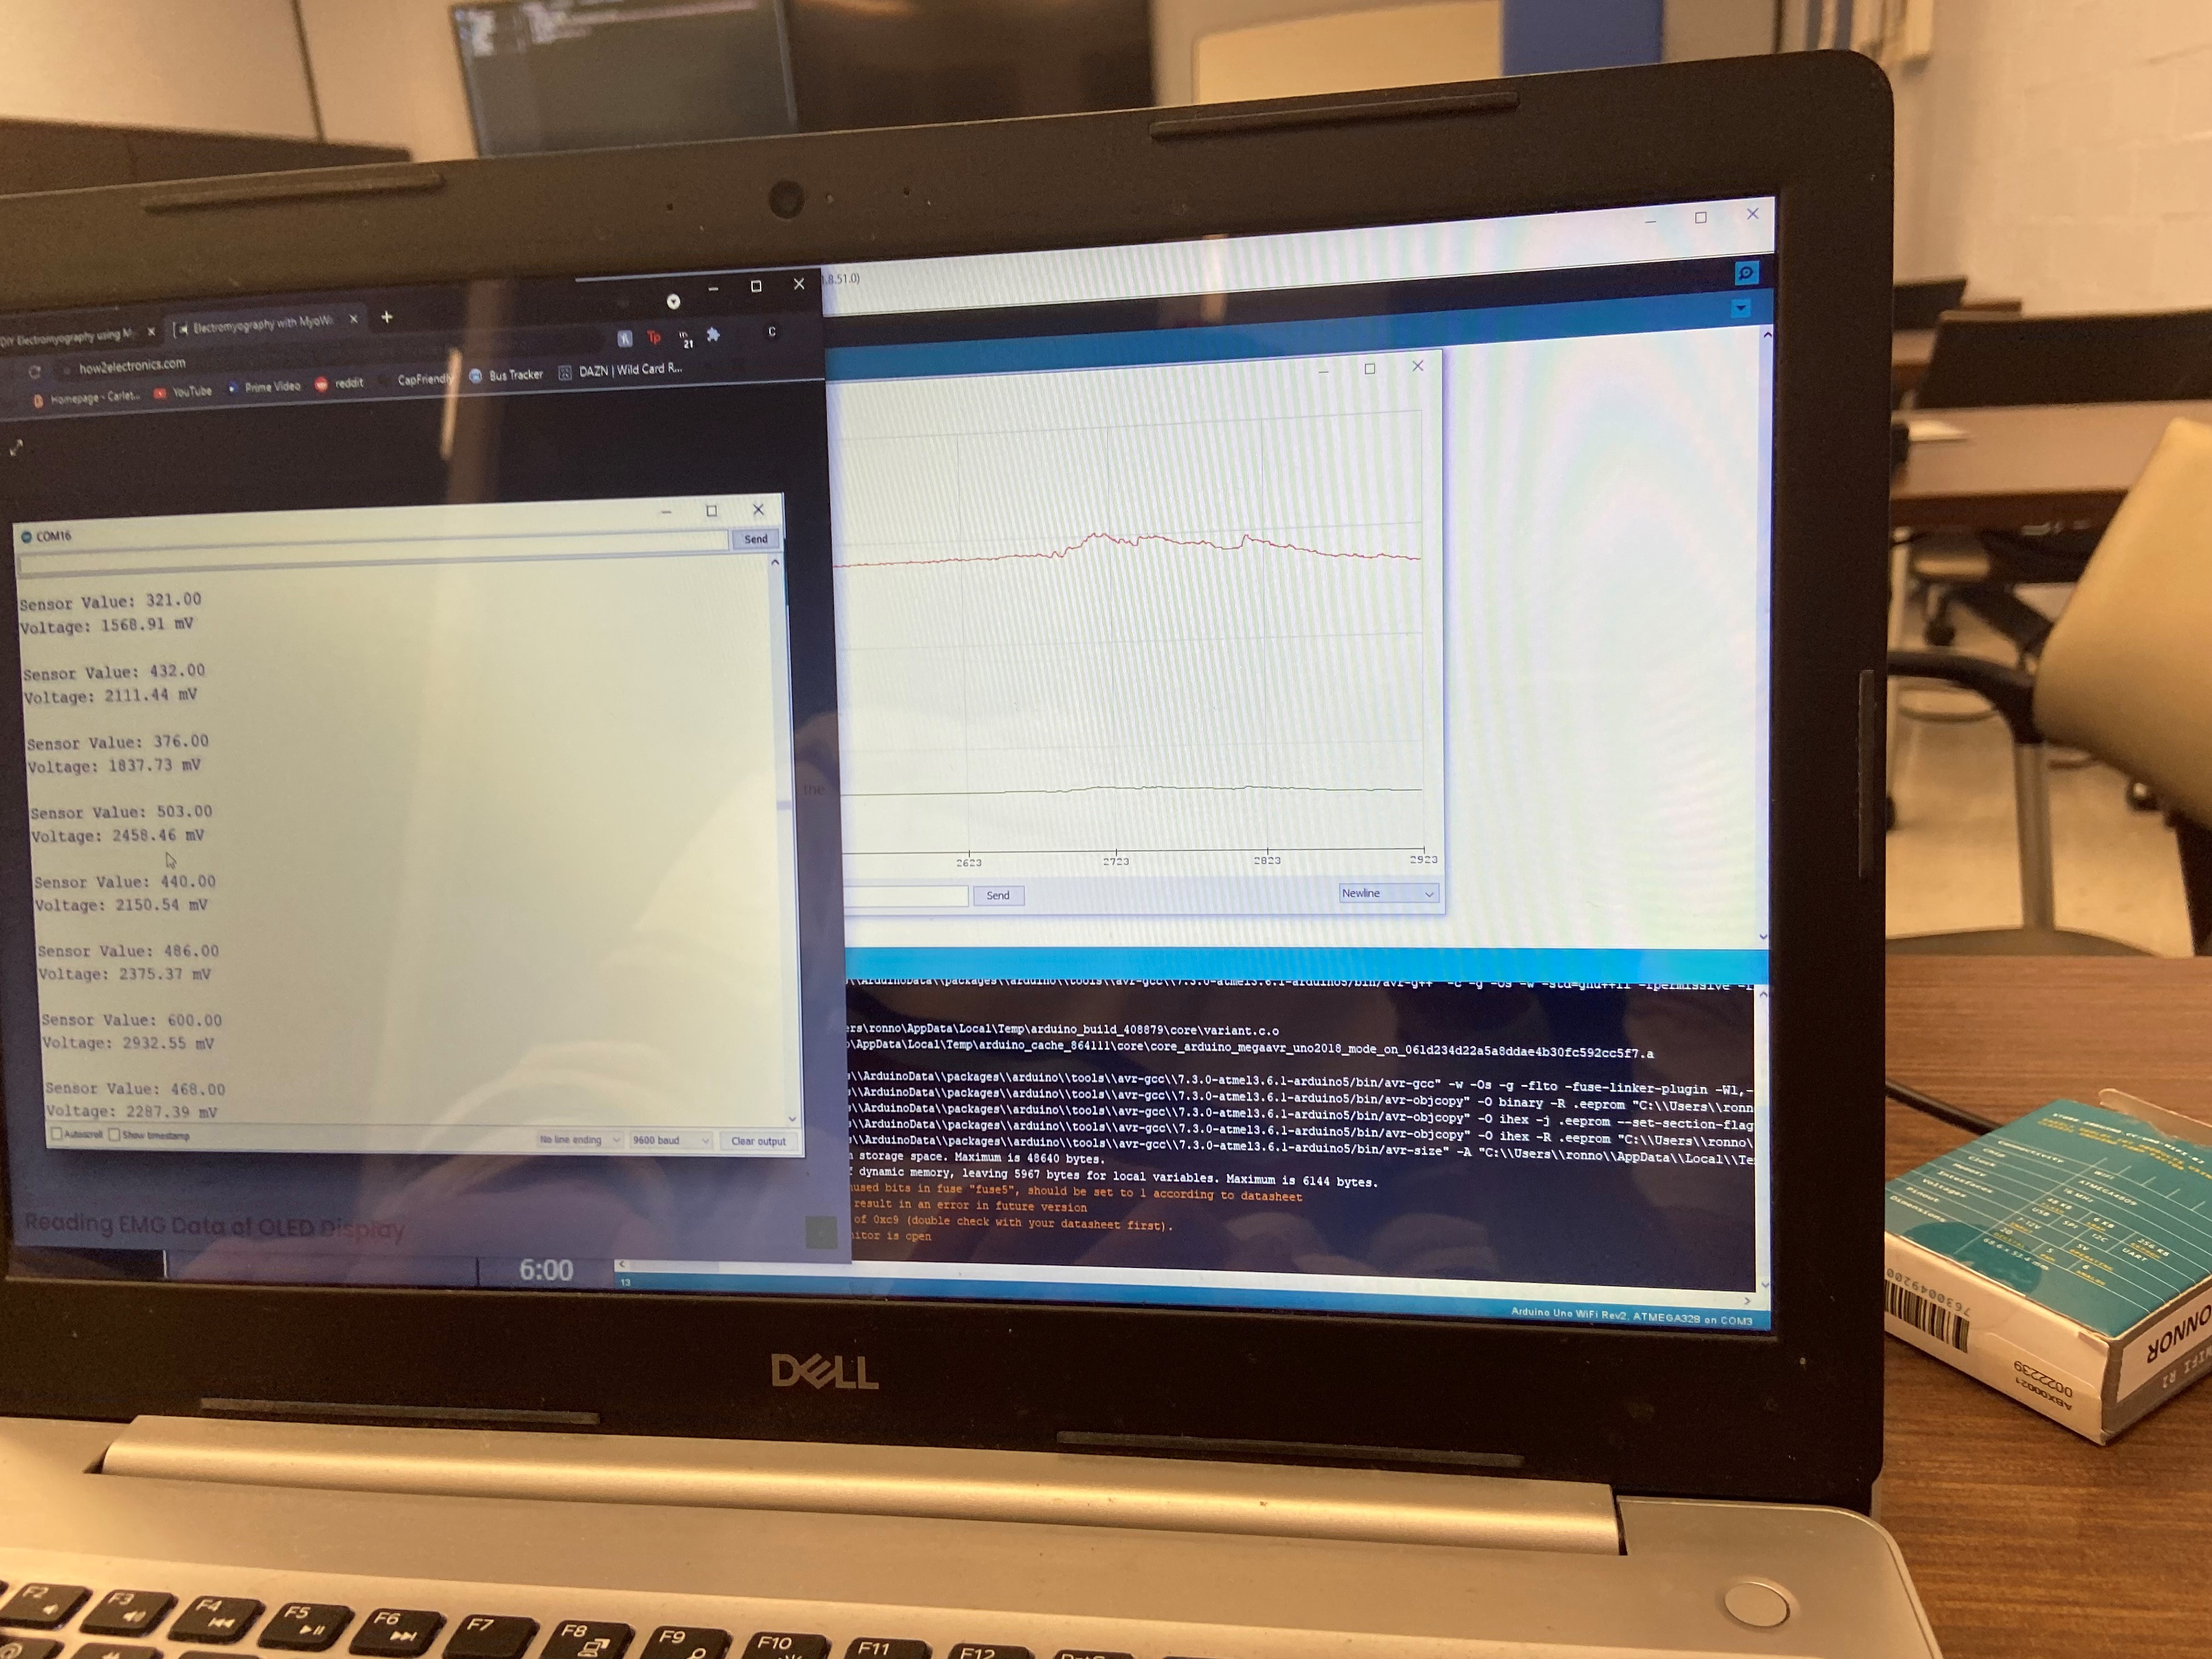
\includegraphics[width=\textwidth]{Progress_Report/figs/EmgReadings.jpg}
         \caption{List of data that was gathered}
         \label{fig:EMG Readings}
     \end{subfigure}
     \hfill
     \begin{subfigure}[h]{0.45\textwidth}
         \centering
         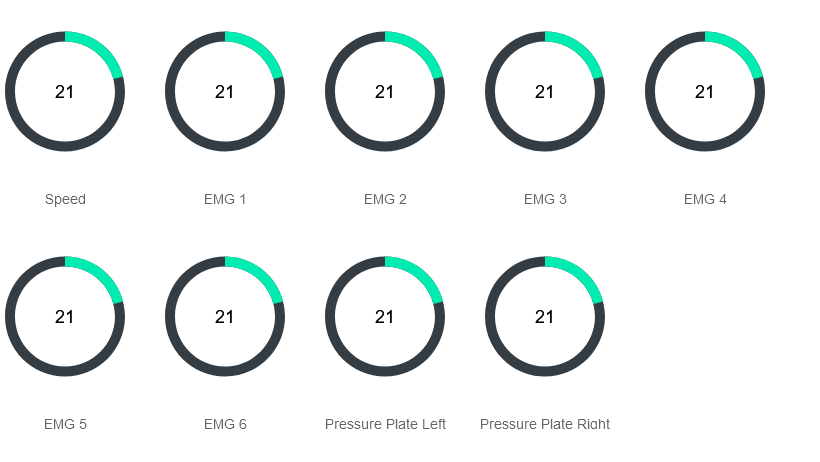
\includegraphics[width=\textwidth]{Progress_Report/figs/emgs.png}
         \caption{Gauges for real time viewing}
         \label{fig:emg gauges}
     \end{subfigure}
     \hfill
     \begin{subfigure}[h]{0.45\textwidth}
         \centering
         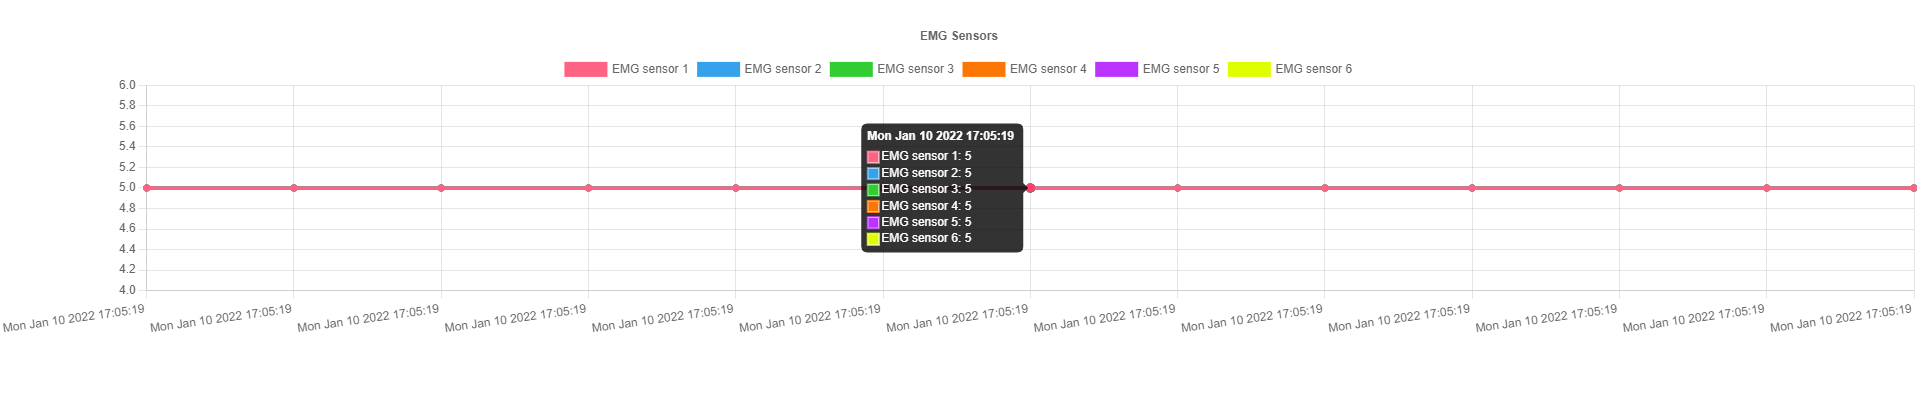
\includegraphics[width=\textwidth]{Progress_Report/figs/graph.png}
         \caption{graph showing data gathered from the EMG sensors.}
         \label{fig:graph}
     \end{subfigure}
     \begin{subfigure}[h]{0.45\textwidth}
         \centering
         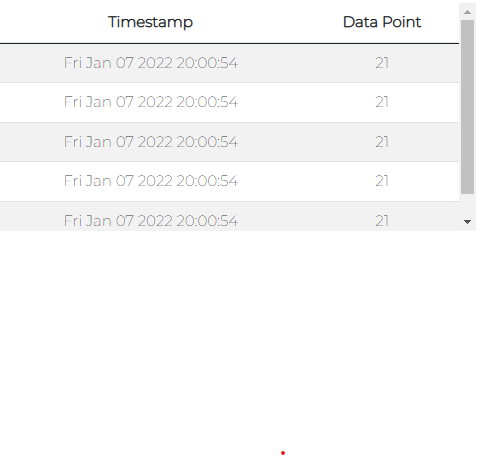
\includegraphics[width=\textwidth]{Progress_Report/figs/data_table.png}
         \caption{Data Table}
         \label{fig:table}
     \end{subfigure}     
        \caption{Software output}
        \label{fig:three graphs}
\end{figure}



